\documentclass{ctacn}
\usepackage{hhline}
\usepackage{threeparttable}
\usepackage{hyperref}
\usepackage{subfigure}

\newcommand{\zhnauthora}{张航宁}
\newcommand{\zhnauthorb}{}
\newcommand{\zhnauthorc}{}
\newcommand{\zhncntitle}{火星气动捕获的建模、制导与仿真}
\newcommand{\zhnentitle}{(Undetermined)Precision of hybrid simulations in modeling numerical solvers}
\newcommand{\zhncnabstract}{本文复现文献\cite{dqingyuan2019},公开版本见\cite{jqingyuan2019guidance,jqingyuan2019coefficient,jqingyuan2019observer}。}
\newcommand{\zhncnkeyword}{火星大气;气动捕获制导;全系数自适应;数值预测校正;鲁棒性}
\newcommand{\zhnenabstract}{This article is designed to help in the contribution for Control and Decision. It is divided into several sections. It consists of the styles and notes for the main text, the mathematical writing style and the topic of drawing tables and inserting figures respectively. The residuals deal with references, acknowledges, etc.}
\newcommand{\zhnenkeyword}{Mars atmosphere; aerocapture guidance; all-coefficient adaptive; numerical predictor-corrector; robustness}

\begin{document}

%%%%%%%
\cndoi{}
\doi{\zihao{-5}10.13195/j.kzyjc.2019.0000}
\paperdate{2018-xx-xx}{2019-xx-xx}%接收日期,修回日期
\osid{}
\setcounter{page}{1}

%%%%%%%%%%
%%%%%%%输入页眉显示的题目
%%%%%%%%%%%%
\runheading{\zhnauthora~等: \zhncntitle}%页眉设置,填写第一作者及论文题目
\xiangmujijin{本文得到国家重点研发计划(批准号:2018YFA0703800), 空间智能控制技术重点实验室基金资助(编号:ZDSYS-2018-04), 和国家自然科学基金(批准号:U20B2054)项目资助。}%项目基金  为空会自动取消显示
\authorcor{E-mail: yz37zhn@163.com.}%通讯作者邮箱,新投稿不修改
\cntitle{\zhncntitle}  % 输入中文标题
\entitle{\zhnentitle}


%                  新投稿不要修改下面的姓名及单位
%%%中文作者和单位,\dag代表通信作者,“作者一”代表3个字的名,“作者”代表2个字的名
\cnauthor{\zhnauthora\makebox{$^{1\dag}$}}  %新投稿不修改
{(北京控制工程研究所,北京100094)}  %%省会城市无需加省%%新投稿不要修改

%%%中文摘要
\cnabstract{\zhncnabstract}

%%%中文关键词
\cnkeyword{\zhncnkeyword}

%%%分类号、标识码
\clc{}  % 中文分类号,请作者自行查找并填写
\wenxianbiaoshi{A}  % 文献标志码

\citation{\zhnauthora. \zhncntitle\hspace{0pt}[J].~期刊名称,~xxxx,~xx(x):~1-xxxx.}

%%%%%%%              新投稿不要修改下面的英文名及单位
\enauthor{Hangning Zhang\makebox{$^{1\dag}$}}{
(1. China Academy of Space Technology,Beijing~100094,China)}
\enabstract{\zhnenabstract}
\enkeyword{\zhnenkeyword}
\maketitle

\begin{multicols}{2}

%%%%%%%%%%%%%%%%%%%%%%%%%%%%%%%%%%%%%%%%%%%%%%%%%%%%%%%%%%%%%%%%
% 正文
%%%%%%%%%%%%%%%%%%%%%%%%%%%%%%%%%%%%%%%%%%%%%%%%%%%%%%%%%%%%%%%%
\section{引\quad 言}
气动捕获制导的总体思路是,
通过不断预测以当前控制量飞出大气后的过渡轨道状态向量与目标轨道的状态向量间的误差,
代入制导算法来产生新的控制量,
如此往复,直到满足终端需求为止。

\section{基本公式推导}
下面推导常用的一些公式。

% ////////////////////////////////////////
\subsection{角速度公式}
设一向量$\vec{x}(t)$绕旋转轴$\vec{\omega}$作匀速圆周运动,
则$\vec{x}(t)$的线速度为
\[\dot{\vec{x}}(t)=\vec{\omega}\times\vec{x}(t)\]
\textbf{证明}:由罗德里格斯((Rodrigues)旋转公式
\[R=\cos\theta I+(1-\cos\theta)\vec{n}\vec{n}^\text{T}+\sin\theta\vec{n}^{\wedge}\]
其中
$R$为旋转矩阵,
$n$为单位旋转轴,
$\theta$为旋转角度,
$\vec{n}^{\wedge}$表示向量$\vec{n}$叉乘对应的反对称矩阵。
将向量$\vec{\omega}$写成$\vec{\omega}=\omega\vec{n}$,
并将旋转矩阵对时间$t$求导得到
\begin{align*}
    \frac{\text{d}}{\text{d}t}R(t)
    =& \frac{\text{d}}{\text{d}t}\left(
        \cos\omega t I
        +(1-\cos\omega t)\frac{\vec{\omega}}{\omega}\frac{\vec{\omega}^\text{T}}{\omega}
        +\sin\omega t\frac{\vec{\omega}^{\wedge}}{\omega}
    \right) \\
    =& -\omega\sin\omega tI
        +\frac{\sin\omega t}{\omega}\vec{\omega}\vec{\omega}^\text{T}
        +\cos\omega t\cdot\vec{\omega}^{\wedge} \\
    \dot{R}(t)\vec{x}_0
    =& -\omega\sin\omega t\vec{x}_0
        +\frac{\sin\omega t}{\omega}\vec{\omega}^\text{T}\vec{x}_0\vec{\omega}
        +\cos\omega t\cdot\vec{\omega}\times\vec{x}_0
\end{align*}
另因为
\begin{align*}
    \vec{\omega}\times R(t)\vec{x}_0
    =& \cos\omega t\cdot\vec{\omega}\times\vec{x}_0
        +\frac{1-\cos\omega t}{\omega^2}\vec{\omega}\times\vec{\omega}\vec{\omega}^\text{T}\vec{x}_0 \\
        &+ \frac{\sin\omega t}{\omega}\vec{\omega}\times(\vec{\omega}\times\vec{x}_0) \\
    =& \cos\omega t\cdot\vec{\omega}\times\vec{x}_0
        +\frac{\sin\omega t}{\omega}(\vec{\omega}^\text{T}\vec{x}_0\vec{\omega}
        -\vec{\omega}^\text{T}\vec{\omega}\vec{x}_0)
\end{align*}
所以
\[\dot{\vec{x}}(t)=\dot{R}(t)\vec{x}_0=\vec{\omega}\times R(t)\vec{x}_0=\vec{\omega}\times\vec{x}(t)\]

% ////////////////////////////////////////
\subsection{旋转坐标系下的速度和加速度}
旋转坐标系$\mathcal{F}_2$绕惯性坐标系$\mathcal{F}_1$以角速度$\vec{\omega}$旋转,
设$\mathcal{F}_1$下位置向量的一阶导和二阶导分别为
$\dot{\vec{r}}$和$\ddot{\vec{r}}$,
$\mathcal{F}_2$下位置向量的一阶导和二阶导为
$\overset{\circ}{\vec{r}}$和$\overset{\circ\circ}{\vec{r}}$,
满足
\begin{align*}
    \dot{\vec{r}}
    =& \overset{\circ}{\vec{r}}
    + \vec{\omega}\times\vec{r} \\
    \ddot{\vec{r}}
    =& \overset{\circ\circ}{\vec{r}}
    + 2\vec{\omega}\times\overset{\circ}{\vec{r}}
    + \overset{\circ}{\vec{\omega}}\times\vec{r}
    + \vec{\omega}\times(\vec{\omega}\times\vec{r})
\end{align*}
\textbf{证明}:
设同一向量$\vec{r}$在坐标系$\mathcal{F}_1$和$\mathcal{F}_2$下的坐标分别为
\begin{equation*}
    \vec{r} = \left[\begin{matrix}
        \vec{e}_x & \vec{e}_y & \vec{e}_z
    \end{matrix}\right]
    \left[\begin{matrix}
        x_1 \\ y_1 \\ z_1
    \end{matrix}\right]
    = \left[\begin{matrix}
        \vec{a}_x & \vec{a}_y & \vec{a}_z
    \end{matrix}\right]
    \left[\begin{matrix}
        x_2 \\ y_2 \\ z_2
    \end{matrix}\right]
\end{equation*}
其中$[\vec{e}_x\ \vec{e}_y\ \vec{e}_z]$表示惯性坐标系$\mathcal{F}_1$下的三轴单位向量,
$[\vec{a}_x\ \vec{a}_y\ \vec{a}_z]$表示坐标系$\mathcal{F}_2$的三轴单位向量在惯性坐标系$\mathcal{F}_1$下的坐标,
三个单位向量张成旋转坐标系$\mathcal{F}_2$,
则向量$\vec{r}$的一阶导
\begin{align*}
    \dot{\vec{r}}
    =& \left[\begin{matrix}
        \dot{\vec{a}}_x & \dot{\vec{a}}_y & \dot{\vec{a}}_z
    \end{matrix}\right]
    \left[\begin{matrix}
        x_2 \\ y_2 \\ z_2
    \end{matrix}\right]
    + \left[\begin{matrix}
        \vec{a}_x & \vec{a}_y & \vec{a}_z
    \end{matrix}\right]
    \left[\begin{matrix}
        \dot{x}_2 \\ \dot{y}_2 \\ \dot{z}_2
    \end{matrix}\right] \\
    =& \vec{\omega}\times
    \left[\begin{matrix}
        \vec{a}_x & \vec{a}_y & \vec{a}_z
    \end{matrix}\right]
    \left[\begin{matrix}
        x_2 \\ y_2 \\ z_2
    \end{matrix}\right]
    + \overset{\circ}{\vec{r}} \\
    =& \vec{\omega}\times\vec{r} + \overset{\circ}{\vec{r}}
\end{align*}
使用坐标系的记法写作
\begin{align*}
    \dot{\vec{r}}
    =& \frac{\text{d}}{\text{d}t}(\mathcal{F}_2\vec{r}_2) \\
    =& \mathcal{F}_2\dot{\vec{r}}_2
    + \dot{\mathcal{F}_2}\vec{r}_2 \\
    =& \mathcal{F}_2\dot{\vec{r}}_2
    + \vec{\omega} \times \mathcal{F}_2\vec{r}_2 \\
    =& \mathcal{F}_2\dot{\vec{r}}_2
    + \vec{\omega} \times \mathcal{F}_1\vec{r}_1
\end{align*}
对上式进一步求导得
\begin{align*}
    \ddot{\vec{r}}
    =& \vec{\omega} \times \mathcal{F}_2\dot{\vec{r}}_2
    + \mathcal{F}_2\ddot{\vec{r}}_2
    + \dot{\vec{\omega}} \times \mathcal{F}_1\vec{r}_1 \\
    &+ \vec{\omega} \times (\vec{\omega} \times \mathcal{F}_2\vec{r}_2
    + \mathcal{F}_2\dot{\vec{r}}_2) \\
    =& \mathcal{F}_2\ddot{\vec{r}}_2
    + 2\vec{\omega} \times \mathcal{F}_2\dot{\vec{r}}_2 \\
    &+ \dot{\vec{\omega}} \times \mathcal{F}_1\vec{r}_1
    + \vec{\omega} \times (\vec{\omega} \times \mathcal{F}_1\vec{r}_1) \\
    =& \overset{\circ\circ}{\vec{r}}
    + 2\vec{\omega}\times\overset{\circ}{\vec{r}}
    + \dot{\vec{\omega}}\times\vec{r}
    + \vec{\omega}\times(\vec{\omega}\times\vec{r})
\end{align*}
其中$\vec{\omega}$在两个坐标系下的坐标相等,
即$\dot{\vec{\omega}}=\overset{\circ}{\vec{\omega}}$。

% ////////////////////////////////////////////////////////////////
\subsection{轨道六根数和位置速度向量}
轨道六根数指:
半长轴(a)、偏心率(e),轨道倾角(i),升交点赤经($\Omega$)、近地点幅角($\omega$)、真近点角($\phi$)。
根据文献\cite{mruiter2012}中的公式计算相关参数。
根据平近点角计算真近点角\cite{msmart1977}
\begin{align*}
    f =& M+\left(2e-{\frac {1}{4}}e^{3}\right)\sin {M}
    + {\frac {5}{4}}e^{2}\sin {2M} \\
    &+ {\frac {13}{12}}e^{3}\sin {3M}+O(e^{4})
\end{align*}

%%%%%%%%%%%%%%%%%%%%%%%%%%%%%%%%%%%%%%%%%%%%%%%%%%%%%%%%%%%%%%%%
% Model
%%%%%%%%%%%%%%%%%%%%%%%%%%%%%%%%%%%%%%%%%%%%%%%%%%%%%%%%%%%%%%%%
\section{飞行器再入动力学方程}
本节推导不考虑火星自转时的飞行器再入制导的动力学方程,
假设飞行器只受空气动力和重力,无风干扰。

首先建立坐标系\cite{mdelong2006}。

1. 火星赤道惯性坐标系($OX_IY_IZ_I$):
原点$O$位于火星球心,
$OX_I$轴指向火星赤道平面与黄道平面相交节线的升交点,
$OZ_I$轴垂直于赤道平面指向北极,
$OY_I$轴与$OX_I$和$OZ_I$轴组成右手正交坐标系。
该坐标系与地球赤道惯性坐标系定义相仿。

2. 火星赤道固连坐标系($OXYZ$):
原点$O$位于火星球心,
$OX$轴在赤道平面内指向零经度线,
$OZ$轴垂直于赤道平面指向北极,
$OY$轴与$OX$和$OZ$轴组成右手正交坐标系。
该坐标系与火星固连,
并相对火星赤道惯性坐标系以火星自转角速度$\omega$转动。

3. 飞行器位置坐标系($Oxyz$):
又称"天东北坐标系",
原点$O$位于火星球心,
$Ox$轴指向飞行器质心$M$,
$Oy$轴在赤道平面与$Ox$轴垂直,
$Oz$轴与$Ox$和$Oy$轴组成右手正交坐标系。

4. 飞行器速度坐标系($Mx_vy_vz_v$):
原点$M$位于飞行器质心,
$Mx_v$轴平行于$Ox$轴,
$Mz_v$轴指向飞行器速度方向,
$My_v$轴与$Mx_v$和$Mz_v$轴组成右手正交坐标系。

气动飞行期间轨道动力学建立在火星赤道固连坐标系$O-XYZ$下,
状态变量定义为:
\[[r\quad\theta\quad\phi\quad V\quad\gamma\quad\psi]\]
其中,
$r$为飞行器距球心的距离,
$\theta$为飞行器当前经度,向东为正,
$\phi$为飞行器当前纬度,向北为正,
$V$为火星赤道固连坐标系下的速度大小,
$\gamma$和$\psi$分别为航迹角和航向角。
航迹角定义为飞行器速度向量与当地水平面的夹角,
速度方向沿铅锤面向上为正;
航向角定义为当地东向与飞行器速度向量在当地水平面的投影的夹角,
速度方向向北偏为正。

飞行器在三维空间中的运动可以由
位置$\vec{r}(t)$和
速度$\vec{v}(t)$两个向量来表征。

用$\vec{i}$,$\vec{j}$,$\vec{k}$分别表示位置坐标系$Oxyz$的三轴单位向量在固连坐标系$OXYZ$下的坐标,
与前文中的$\vec{a}_x$,$\vec{a}_y$,$\vec{a}_z$表示类似,
则固连坐标系下的位置向量$\vec{r}$、速度向量$\vec{V}$、火星角速度向量$\vec{\omega}$分别表示成位置坐标系下的向量为
\begin{align}
    \vec{r} =& r\vec{i} \label{eqModelr}\\
    \vec{V} =& V\sin\gamma\vec{i} + V\cos\gamma\cos\psi\vec{j} + V\cos\gamma\sin\psi\vec{k} \label{eqModelV}\\
    \vec{\omega} =& \omega\sin\phi\vec{i} + \omega\cos\phi\vec{k} \notag
\end{align}
举例说明,
用$\vec{e}_x$,$\vec{e}_y$,$\vec{e}_z$分别表示固连坐标系$OXYZ$的三轴单位向量在固连坐标系下的坐标,
即$[\vec{e}_x\ \vec{e}_y\ \vec{e}_z]$为单位矩阵,
则速度向量式\eqref{eqModelV}可以表示为
\begin{equation*}
    \vec{V}
    =\left[\begin{matrix}
        \vec{e}_x & \vec{e}_y & \vec{e}_z
    \end{matrix}\right]
    \left[\begin{matrix}
        V_x \\ V_y \\ V_z
    \end{matrix}\right]
    =\left[\begin{matrix}
        \vec{i} & \vec{j} & \vec{k}
    \end{matrix}\right]
    \left[\begin{matrix}
        V\sin\gamma \\ V\cos\gamma\cos\psi \\ V\cos\gamma\sin\psi
    \end{matrix}\right]
\end{equation*}

坐标系$Oxyz$是坐标系$OXYZ$绕$OZ$轴正向转动$\theta$角,然后绕$Oy$轴负向转动$\phi$角得到的,
因此,坐标系$Oxyz$绕坐标系$OXYZ$的角速度大小$\Omega$为
\[\Omega = \dot{\theta} + \dot{\phi}\]
位置坐标系$Oxyz$下的角速度向量$\vec{\Omega}$为
\[\vec{\Omega} = \dot{\theta}\sin\phi\vec{i} - \dot{\phi}\vec{j} +\dot{\theta}\cos\phi\vec{k}\]
由此可以得出$\vec{i}$,$\vec{j}$,$\vec{k}$相对固连坐标系$OXYZ$的时间导数
\begin{align*}
    \frac{\text{\text{\text{\text{\text{d}}}}}\vec{i}}{\text{\text{\text{\text{\text{d}}}}}t} &=\vec{\omega} \times \vec{i}
    =  \left(\cos \phi \frac{\text{\text{\text{\text{\text{d}}}}}\theta}{\text{\text{\text{\text{\text{d}}}}}t}\right) \vec{j}
    + \left(\frac{\text{\text{\text{\text{\text{d}}}}}\phi}{\text{\text{\text{\text{\text{d}}}}}t}\right) \vec{k} \\
    \frac{\text{d}\vec{j}}{\text{d}t} &=\vec{\omega} \times \vec{j}
    = -\left(\cos \phi \frac{\text{d}\theta}{\text{d}t}\right) \vec{i}
    + \left(\sin \phi \frac{\text{d}\theta}{\text{d}t}\right) \vec{k} \\
    \frac{\text{d}\vec{k}}{\text{d}t} &=\vec{\omega} \times \vec{k}
    = -\left(\frac{\text{d}\phi}{\text{d}t}\right) \vec{i}
    - \left(\sin \phi \frac{\text{d}\theta}{\text{d}t}\right) \vec{j}
\end{align*}
式\eqref{eqModelr}求导得到速度
\[
    \vec{V}=\frac{\text{d}\vec{r}}{\text{d}t}
    =\left(\frac{\text{d}r}{\text{d}t}\right)\vec{i}
    +\left(r\cos\phi\frac{\text{d}\theta}{\text{d}t}\right)\vec{j}
    +\left(r\frac{\text{d}\phi}{\text{d}t}\right)\vec{k}
\]
与式\eqref{eqModelV}比较可得到
\begin{align*}
    \frac{\text{d}r}{\text{d}t} &=V\sin\gamma \\
    \frac{\text{d}\theta}{\text{d}t}&=\frac{V\cos\gamma\sin\psi}{r\cos\phi} \\
    \frac{\text{d}\phi}{\text{d}t}&=\frac{V\cos\gamma\cos\psi}{r}
\end{align*}
对$\vec{V}$求导可以得到
\begin{align*}
    \frac{d \vec{V}}{d t}=& {\left[\sin \gamma \frac{d V}{d t}+V \cos \gamma \frac{d \gamma}{d t}-\frac{V^{2}}{r} \cos ^{2} \gamma\right] \vec{i} } \\
    &+\left[\cos \gamma \sin \psi \frac{d V}{d t}-V \sin \gamma \sin \psi \frac{d \gamma}{d t}+V \cos \gamma \cos \psi \frac{d \psi}{d t}\right.\\
    &\left.+\frac{V^{2}}{r} \cos \gamma \sin \psi(\sin \gamma-\cos \gamma \cos \psi \tan \phi)\right] \vec{j} \\
    &+\left[\cos \gamma \cos \psi \frac{d V}{d t}-V \sin \gamma \cos \psi \frac{d \gamma}{d t}-V \cos \gamma \sin \psi \frac{d \psi}{d t}\right.\\
    &\left.+\frac{V^{2}}{r} \cos \gamma\left(\sin \gamma \cos \psi+\cos \gamma \sin ^{2} \psi \tan \phi\right)\right] \vec{k}
\end{align*}

气动力的升力和阻力表达式为
\begin{equation*}
    \left[\begin{matrix}
        L \\ D
    \end{matrix}\right]
    = \frac{1}{2}\rho V^2S_{\text{ref}}
    \left[\begin{matrix}
        C_L \\ C_D
    \end{matrix}\right]
\end{equation*}
其中,
$\rho$为火星大气密度,
$S_{\text{ref}}$为飞行器的气动参考面积,
$C_L$、$C_D$分别为升力系数和阻力系数,
为简化问题可设除了大气密度$\rho$以外其余均为常数。
升力、阻力和速度三个向量位于同一平面内,称为阻力平面。
阻力平面与铅垂面的夹角称为倾侧角$\sigma<90^{\circ}$。
阻力和速度方向相反,
升力在阻力平面内与速度向量垂直,方向向上。

火星大气密度$\rho$在简化大气指数模型中可以用
\[\rho=\rho_0e^{-h/h_s}\]
表示,其中参考密度$\rho_0=1.474\times10^7$kg/km$^2$,
比例高度$h_s=8.8057$km。

%%%%%%%%%%%%%%%%%%%%%%%%%%%%%%%%%%%%%%%%%%%%%%%%%%%%%%%%%%%%%%%%
% Real
%%%%%%%%%%%%%%%%%%%%%%%%%%%%%%%%%%%%%%%%%%%%%%%%%%%%%%%%%%%%%%%%
\section{实时仿真理论}
宇宙中各天体的自转或公转周期通常以天甚至以年计算,
且轨道速度快,空间尺度大。
如果按照实际参数进行仿真,
则仿真的计算量太大而无法实时计算。
为了能够在仿真时直观地实时展示仿真结果,
需要对一些公式的单位进行换算。

万有引力公式
\begin{equation}
    \frac{\text{d}^2\vec{r}}{\text{d}t^2}=-\frac{\mu}{r^3}\vec{r} \label{eqRealGravity}
\end{equation}
中,$r$的单位是km,$t$的单位是s。
因为实际的尺度太大,一个天文单位达到了$10^8$数量级,
为了便于仿真,
需要将实际尺度中的时间和距离变换到一个合适的时空坐标系下。
首先列举一些名词解释。
\textbf{实际时间}指宇宙尺度上的实际时间;
\textbf{无单位求解器时间}指微分方程求解器中自变量的值,
没有单位,简称求解器时间,
对应的求解器速度和求解器距离也都没有单位;
\textbf{仿真展示软件消耗时间}:例如仿真展示软件运行1秒对应实际时间的1000秒,
此处的1秒指的是是仿真展示软件消耗时间,简称展示时间。

举例说明,
求解器时间的1单位时间等于实际时间的$10^4$秒,
1单位距离等于实际距离$10^6$km,即在求解器中,
\begin{equation}
    \bar{t}=10^{-4}t,\ \bar{r}=10^{-6}r \label{eqRealConvert}
\end{equation}
其中$t$和$r$分别为以秒和千米为单位的实际时间和实际距离,
而$\bar{t}$和$\bar{r}$分别表示求解器时间和求解器距离。
1个天文单位为$r=1.5*10^8$km,
则求解器中的1个天文单位为$\bar{r}=150$。
然后可以计算出实际时间/速度/距离
和求解器时间/速度/距离之间的一些换算关系
\begin{align*}
&\bar{v} = \frac{\text{d}\bar{r}}{\text{d}\bar{t}}
 = \frac{10^{-6}\text{d}r}{10^{-4}\text{d}t} = 10^{-2}v \\
&\bar{a} = \frac{\text{d}}{\text{d}\bar{t}}\frac{\text{d}\bar{r}}{\text{d}\bar{t}}
 = 10^2\frac{\text{d}^2r}{\text{d}t^2} = 10^2a \\
&\bar{\mu}\left[\frac{(10^{-6}\text{km})^3}{\text{kg}\cdot(10^{-4}\text{s})^2}\right]
 = 10^{-10}\mu\left[\frac{\text{km}^3}{\text{kg}\cdot \text{s}^2}\right] \\
&-\frac{\bar{\mu}}{\bar{r}^2} = -10^2\frac{\mu}{r^2}
 = 10^2\frac{\text{d}^2r}{\text{d}t^2} = \bar{a}
\end{align*}
其中引力常数$\mu$的单位中包含时间/距离量纲,
因此也需要换算。
可以验证,实际中的微分方程
$$a=-\frac{\mu}{r^2}$$
变换到求解器中仍然为
$$\bar{a}=-\frac{\bar{\mu}}{\bar{r}^2}$$

下面在换算公式\eqref{eqRealConvert}的基础上引入仿真展示软件消耗时间。
若仿真步长设置为0.01求解器时间,仿真展示软件每帧仿真10步,
则换算到实际时间上的步长为100秒,每帧代表1000秒,
按60帧计算,则展示时间1秒等于实际时间$6\times10^4$秒,
地球的轨道速度按30km/s算则展示时间1秒内地球走过$1.8\times10^6$km,
换算回仿真中则走过1.8展示距离。
换一种方法计算,
地球的求解器速度是$\bar{v}=10^{-2}\times30=0.3$,
仿真展示软件每1秒仿真:
60帧$\times$10步/帧$\times$0.01单位时间/步=6个时间单位,
也可以得到展示时间1秒内地球走过1.8展示距离。
在式\eqref{eqRealConvert}的设定下,
仿真展示软件每帧仿真1步与10步对应的地球自转周期分别约为$14.4$和$1.44$秒,
分别可用于展示低轨卫星和地球同步卫星的动态运行结果。

与实时仿真不同的是实际中广泛使用的非实时仿真,
也就是在一次仿真结束后展示静态仿真结果。
此时虽然不需要考虑展示时间/速度/距离,
但求解器时间/速度/距离仍然需要考虑。
本文的火星气动捕获场景中,
火星半径约$3400$km,
全局飞行时间处于约$10^4$秒数量级,
采样点间隔取10秒,
仿真步长取$1e-3$,
则式\eqref{eqRealConvert}中取
$\bar{r}=10^{-3}r$,$\bar{t}=10^{-4}t$,
指求解器1单位距离表示实际距离$10^3$千米,
求解器1单位时间表示实际时间$10^4$秒。
对应的一些变量和常数的换算关系如下
\begin{align*}
    &\bar{v} = 10v \\
    &\bar{a} = 10^5a \\
    &\bar{\mu}\left[\frac{(10^{-3}\text{km})^3}{\text{kg}\cdot(10^{-4}\text{s})^2}\right]
     = 10^{-1}\mu\left[\frac{\text{km}^3}{\text{kg}\cdot \text{s}^2}\right] \\
    &-\frac{\bar{\mu}}{\bar{r}^2} = -10^5\frac{\mu}{r^2} = 10^5a = \bar{a} \\
    &\bar{\rho_0}\left[\frac{\text{kg}}{(10^{-3}\text{km})^3}\right]
    = 10^9\rho_0\left[\frac{\text{kg}}{\text{km}^3}\right] \\
    &\bar{h}_s[10^{-3}\text{km}] = 10^{-3}h_s[\text{km}] \\
    &\bar{S}_\text{ref}[(10^{-3}\text{km})^2] = 10^{-6}S_\text{ref}[\text{km}^2]
\end{align*}
另由量纲运算可得
升力系数和阻力系数的单位为$10^{-3}$,
升阻比无单位,均不需要换算。

如果仿真需要展示系统运动的动态过程,
则应使用实时仿真,否则应使用非实时仿真。
本文中火星气动捕获制导结果仅需要展示最终制导轨迹,
因此使用使用非实时仿真,
不需要考虑展示时间/速度/距离。

另外可以证明单位换算在显著加快仿真速度的条件下,
微分方程数值求解的精度也明显增加。
已知四阶龙格库塔法的局部截断误差为$O(h^5$)\cite{mqingyang2019},
取步长为$h_1=10^{-3}$秒,
仿真10秒的累积误差为
\[e_1=10^4C\times 10^{-15}=10^{-11}C\]
若将时间单位换算成千秒,
取步长$h_2=10^{-3}$千秒,
仿真10秒的累积误差为
\[e_2=10C\times 10^{-15}=10^{-14}C\]
若不换算单位而只是改变步长,
取步长$h_3=1$秒,
尽管$h_3=h_2$,
但累积误差高达
\[e_3=10C\times 1=10C\]
因此在不同的仿真中,
为了保证仿真速度和精度,
需要保持仿真步长基本不变,
而由此带来的仿真步长与仿真时间不匹配的情况
应使用单位换算的方法解决。

%%%%%%%%%%%%%%%%%%%%%%%%%%%%%%%%%%%%%%%%%%%%%%%%%%%%%%%%%%%%%%%%
% Sim
%%%%%%%%%%%%%%%%%%%%%%%%%%%%%%%%%%%%%%%%%%%%%%%%%%%%%%%%%%%%%%%%
\section{仿真}

% ////////////////////////////////////////
\subsection{被控对象建模}
可以用上一节中推导出的式\eqref{eqModelTotal}建立被控对象微分方程,
若忽略火星自转的影响,
也可以建立向量形式的微分方程
\begin{equation}
    \ddot{\vec{r}} = \frac{\mu}{||\vec{r}||^3}\vec{r}+\vec{L}+\vec{D} \label{eqSimFA}
\end{equation}
其中阻力向量为
\begin{align}
    \vec{D} = -D\frac{\vec{v}}{||\vec{v}||} \label{eqSimFD}
\end{align}
升力向量$\vec{L}$与铅垂面夹角为倾侧角$\sigma$,
为了能将$\vec{L}$用其他已知向量表示,
需要构造一对与$\vec{L}$同平面的正交单位向量。
已知$\vec{v}$与$\vec{r}$张成铅垂面,
另构造一个垂直于铅垂面且在惯性系中方向向上的单位向量$\vec{n}_2$,
和另一个与$\vec{r}$同方向的单位向量$\vec{n}_1$,
则$\vec{n}_1$位于铅垂面内,
此时$\vec{L}$与$\vec{n}_1$的夹角即为倾侧角,
$\vec{n}_1$和$\vec{n}_2$即为用于表示$\vec{L}$的正交单位向量,
即
\begin{align}
    \vec{n}_2 =& \frac{\vec{r}\times\vec{v}}{||\vec{r}\times\vec{v}||} \notag\\
    \vec{L}=\vec{n}_1\cos\sigma + \vec{n}_2\sin\sigma \label{eqSimFL}
\end{align}
% 在升力系数$C_L$和阻力系数$C_D$均为常数的假设下,
% 升力向量$\vec{L}$和阻力向量$\vec{D}$的夹角保持不变,
微分方程式\eqref{eqSimFA}\eqref{eqSimFD}\eqref{eqSimFL}共同组成被控对象模型。
建立飞行器被控对象模型的模块框图如图\ref{figSimPlant}所示。
\begin{center}
	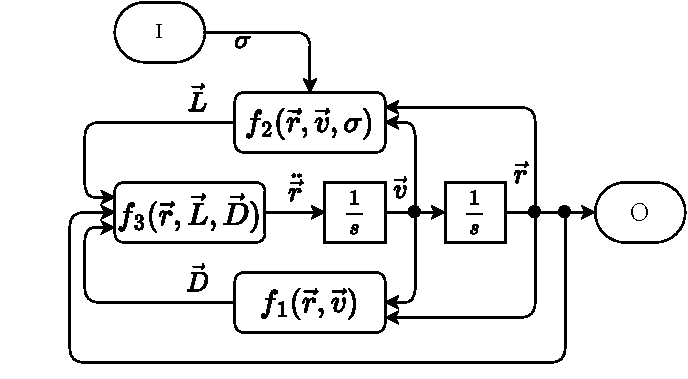
\includegraphics[scale=0.8]{plant.pdf}  \\
	\figcaption{被控对象模型的模块框图}\label{figSimPlant}
\end{center}
图中,被控对象的输入(控制量)为倾侧角$\sigma$,
输出为位置$\vec{r}$。
图中的两个多输入单输出函数分别为式\eqref{eqSimFLDTotal}\eqref{eqSimFATotal}
\begin{align}
    \left\{\begin{aligned}
    h =& ||\vec{r}||-R \\
    \rho =& \rho_0e^{-h/h_s} \\
    D =& \frac{1}{2}\rho||\vec{v}||^2S_{\text{ref}}C_D \\
    \vec{D} =& f_1(\vec{r},\vec{v}) = -D\frac{\vec{v}}{||\vec{v}||} \\
    L =& DC_{LD} \\
    \vec{n}_1 =& \frac{\vec{r}}{||\vec{r}||} \\
    \vec{n}_2 =& \frac{\vec{r}\times\vec{v}}{||\vec{r}\times\vec{v}||} \\
    \vec{L} =& f_2(\vec{r},\vec{v},\sigma) = L(\vec{n}_1\cos\sigma + \vec{n}_2\sin\sigma) \\
    \vec{f}_{LD} =& f_{LD}(\vec{r},\vec{v},\sigma) = \vec{L} + \vec{D}
\end{aligned}\right. \label{eqSimFLDTotal}
\end{align}
\begin{equation}
    \ddot{\vec{r}} = f_{LD}(\vec{r},\vec{f}_{LD}) = \frac{\mu}{||\vec{r}||^3}\vec{r}+\vec{f}_{LD} \label{eqSimFATotal}
\end{equation}
式中$R$为火星半径,$C_{LD}=C_L/C_D$为升阻比。

% ////////////////////////////////////////
\subsection{仿真结果}


\section{程序说明}
所有程序使用git版本管理且已上传GitHub和Gitee。 \\
\textbf{报告:}\url{https://github.com/xd15zhn/paperaerocapture} \\
报告使用\LaTeX 编写,编译器为texlive2022/xelatex。\\
\textbf{简化模型:}\url{https://github.com/xd15zhn/aerocapturecpp} \\
使用C++编写时间加快$10^4$倍的简化模型,输入倾侧角为常数时的仿真结果。 \\
\textbf{完整版:}\url{https://github.com/xd15zhn/aerocaptureguide} \\
使用C++编写,加入制导算法。\\
GitHub和Gitee中对应代码仓库的名称相同。
依赖库和各文件的内容等进一步的说明见各自的README.md文件。



\end{multicols}
\end{document}
